\documentclass{article}
\usepackage{graphicx}
\usepackage{subcaption}
\usepackage{amsmath,amssymb,amsthm}
\DeclareMathOperator{\arcsec}{arcsec}
\DeclareMathOperator{\arccot}{arccot}
\DeclareMathOperator{\arccsc}{arccsc}
\usepackage{graphicx,float}\graphicspath{{images/}}
\usepackage{blindtext}
\usepackage{parskip}
\usepackage{MnSymbol}
\usepackage[letterpaper,top=3cm, left= 3cm,bottom=3cm]{geometry}
\numberwithin{equation}{section}

\title{Odd and Even Functions}
\author{Polaris}
\date{2024/12/09}

\begin{document}

\maketitle

\section{Definition}
\subsection{Odd Functions}
A function is said to be odd if:
\begin{equation}
    f(-x) = -f(x)
\end{equation}

The graph of an odd function is symmetrical with respect to $(0,0)$

\begin{figure}[H]
    \centering
    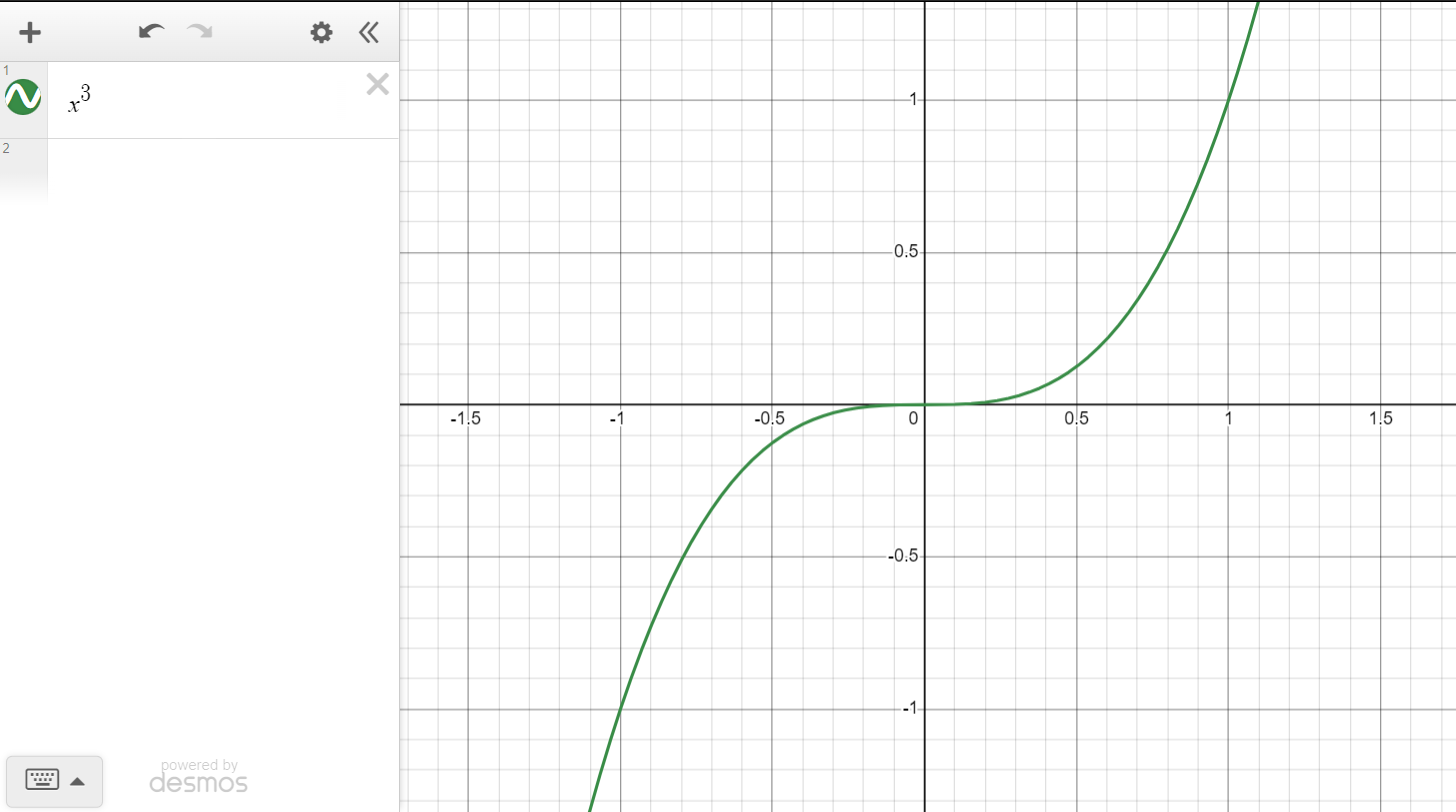
\includegraphics[width = 15cm]{pictures/oddfunction1.png}
    \caption{The graph of $y=x^3$, an odd function}
\end{figure}

\newpage
\subsection{Even function}
A function is said to be even if:
\begin{equation}
    f(x) = f(-x)
\end{equation}

The graph of an even function is symmetrical with respect to the $y$ axis.
\begin{figure}[H]
    \centering
    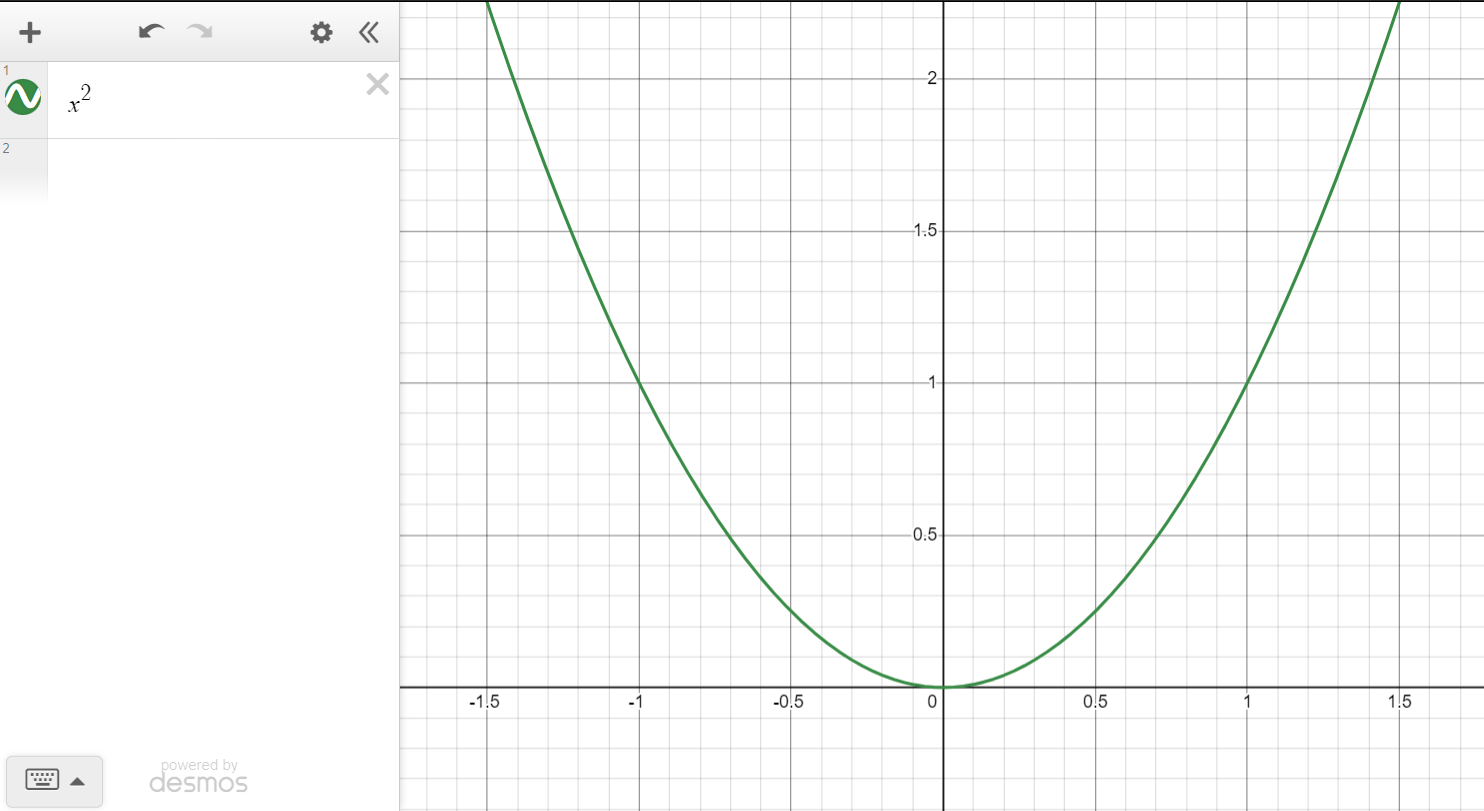
\includegraphics[width = 15cm]{pictures/evenfunction1.png}
    \caption{The graph of $y = x^2$, an even function}
\end{figure}

\section{Properties}
Let $f(x), g(x)$ be odd function, $a(x), b(x)$ be even function

We will first start with the basic properties:
\begin{enumerate}
    \item If a function is both even and odd, it is equal to $0$ everywhere
    \item If a function is odd, the absolute value of that function is even
\end{enumerate}
\subsection{Odd Function}
The properties of odd functions include:
\begin{enumerate}
    \item The sum/difference of two odd functions is odd
    \item The product/quotient of two odd functions is even
    \item The composition of two odd functions is odd: $h(x) = f(g(x))$ is odd
\end{enumerate}
\subsection{Even Function}
\begin{enumerate}
    \item The sum/difference of two even functions is even
    \item The product/quotient of two even functions is even
    \item The composition of two even functions is even: $j(x) = a(b(x))$ is even
\end{enumerate}

\subsection{Odd Function and Even Function}
When calculations are done between an odd function and an even function, the result holds the following properties:
\begin{enumerate}
    \item The sum/difference of an odd function and an even function is not odd or even, unless one of the function equals to $0$
    \item The product/quotient of an odd function and an even function is an odd function
    \item The composition of any function with an even function is even (not vice versa): $k(x) = a(f(x))$ is even
\end{enumerate}

\section{Examples}
\subsection{Odd Function}

\begin{enumerate}
    \item $f(x) = x^n$, where $n$ is an odd number
    \item $f(x) = \sin x, f(x) = \tan x f(x) = \cot x, f(x) = \csc x$
    \item $f(x) = \arcsin x, f(x) = \arctan x, f(x) = \arccsc x$
\end{enumerate}

\subsection{Even Function}
\begin{enumerate}
    \item $f(x) = x^n$, where $n$ is an even number
    \item $f(x) = \cos x, f(x) = \sec x$
\end{enumerate}

\section{In Calculus}
For an odd function $f(x)$, its integral over a symmetrical interval $(-a,a)$ is $0$:
\begin{equation}
    \int_{-a}^a f(x) dx = 0
\end{equation}

For an even function $g(x)$, its integral over a symmetrical interval $(-a,a)$ is $2$ times its integral from $(0,a)$:
\begin{equation}
    \int_{-a}^{a} g(x) dx = 2\int_0^a g(x)dx
\end{equation}
\end{document}